\section{Evaluation with Java Projects}

In this section, we evaluate the precision and recall of our approach using a recently proposed dataset of refactorings performed in real-world Java open source projects. We also compare RefDiff's accuracy with RMiner, 
a state-of-the-art tool for detecting refactorings in Java.
First, we present our evaluation design (Section~\ref{sec:eval:java:design}) and then we present the results (Section~\ref{sec:eval:java:results}).

\subsection{Evaluation Design}
\label{sec:eval:java:design}

To evaluate the precision and recall of RefDiff in Java we initially use an oracle proposed by Tsantalis et al.~\cite{tsantalis2018rminer}.
This oracle includes 3,188 manually-validated refactoring instances, detected in 538 commits from 185 open source projects, and covering 15 refactoring operations.
We also use this oracle to compare RefDiff's precision and recall against RMiner.
For the purpose of the comparison, we restricted the oracle to 11 refactoring types supported by both tools.
Specifically, we excluded \emph{Change Package}, \emph{Move Field}, \emph{Push Down Field} and \emph{Pull Up Field} from the analysis as they are not supported by RefDiff.
Moreover, \emph{Convert Type} and \emph{Change Signature}, although supported by RefDiff, are not evaluated because they are not covered by the oracle.
In total, our modified oracle contains 3,031 confirmed refactoring instances.
Additionally, it also contains 704 refactoring instances classified as false positives in the process of manual validation performed by Tsantalis et al.~\cite{tsantalis2018rminer}.
%Last, it is worth noting that the \emph{Rename Class} category also includes instances of \emph{Move and Rename Class}. Similarly, the \emph{Extract Method} category also includes instances of \emph{Extract and Move Method}. This measure was necessary because the oracle did not distinguish between those refactorings reliably.

First, we run RefDiff on each commit of the oracle. For each detected refactoring $r$ we checked whether $r$ is in the oracle, which may yield three outcomes: (i) if $r$ is a confirmed refactoring from the oracle, then it is a true positive; (ii) if $r$ is a false refactoring from the oracle, then it is a false positive; (iii) otherwise, $r$ was inspected by two authors of this paper to assess whether it is a false positive or a true positive not covered by the oracle.
This extra manual validation is needed because the initial oracle must not be granted as complete, i.e., including all refactorings performed in the set of analysed commits.
Specifically, this oracle was constructed using a triangulation approach, based on an initial list of refactorings produced by RMiner and RefDiff 1.0. For this reason, it might miss true refactorings only detected by the improved implementation of RefDiff, described in this paper.

\begin{figure*}[!t]
\centering
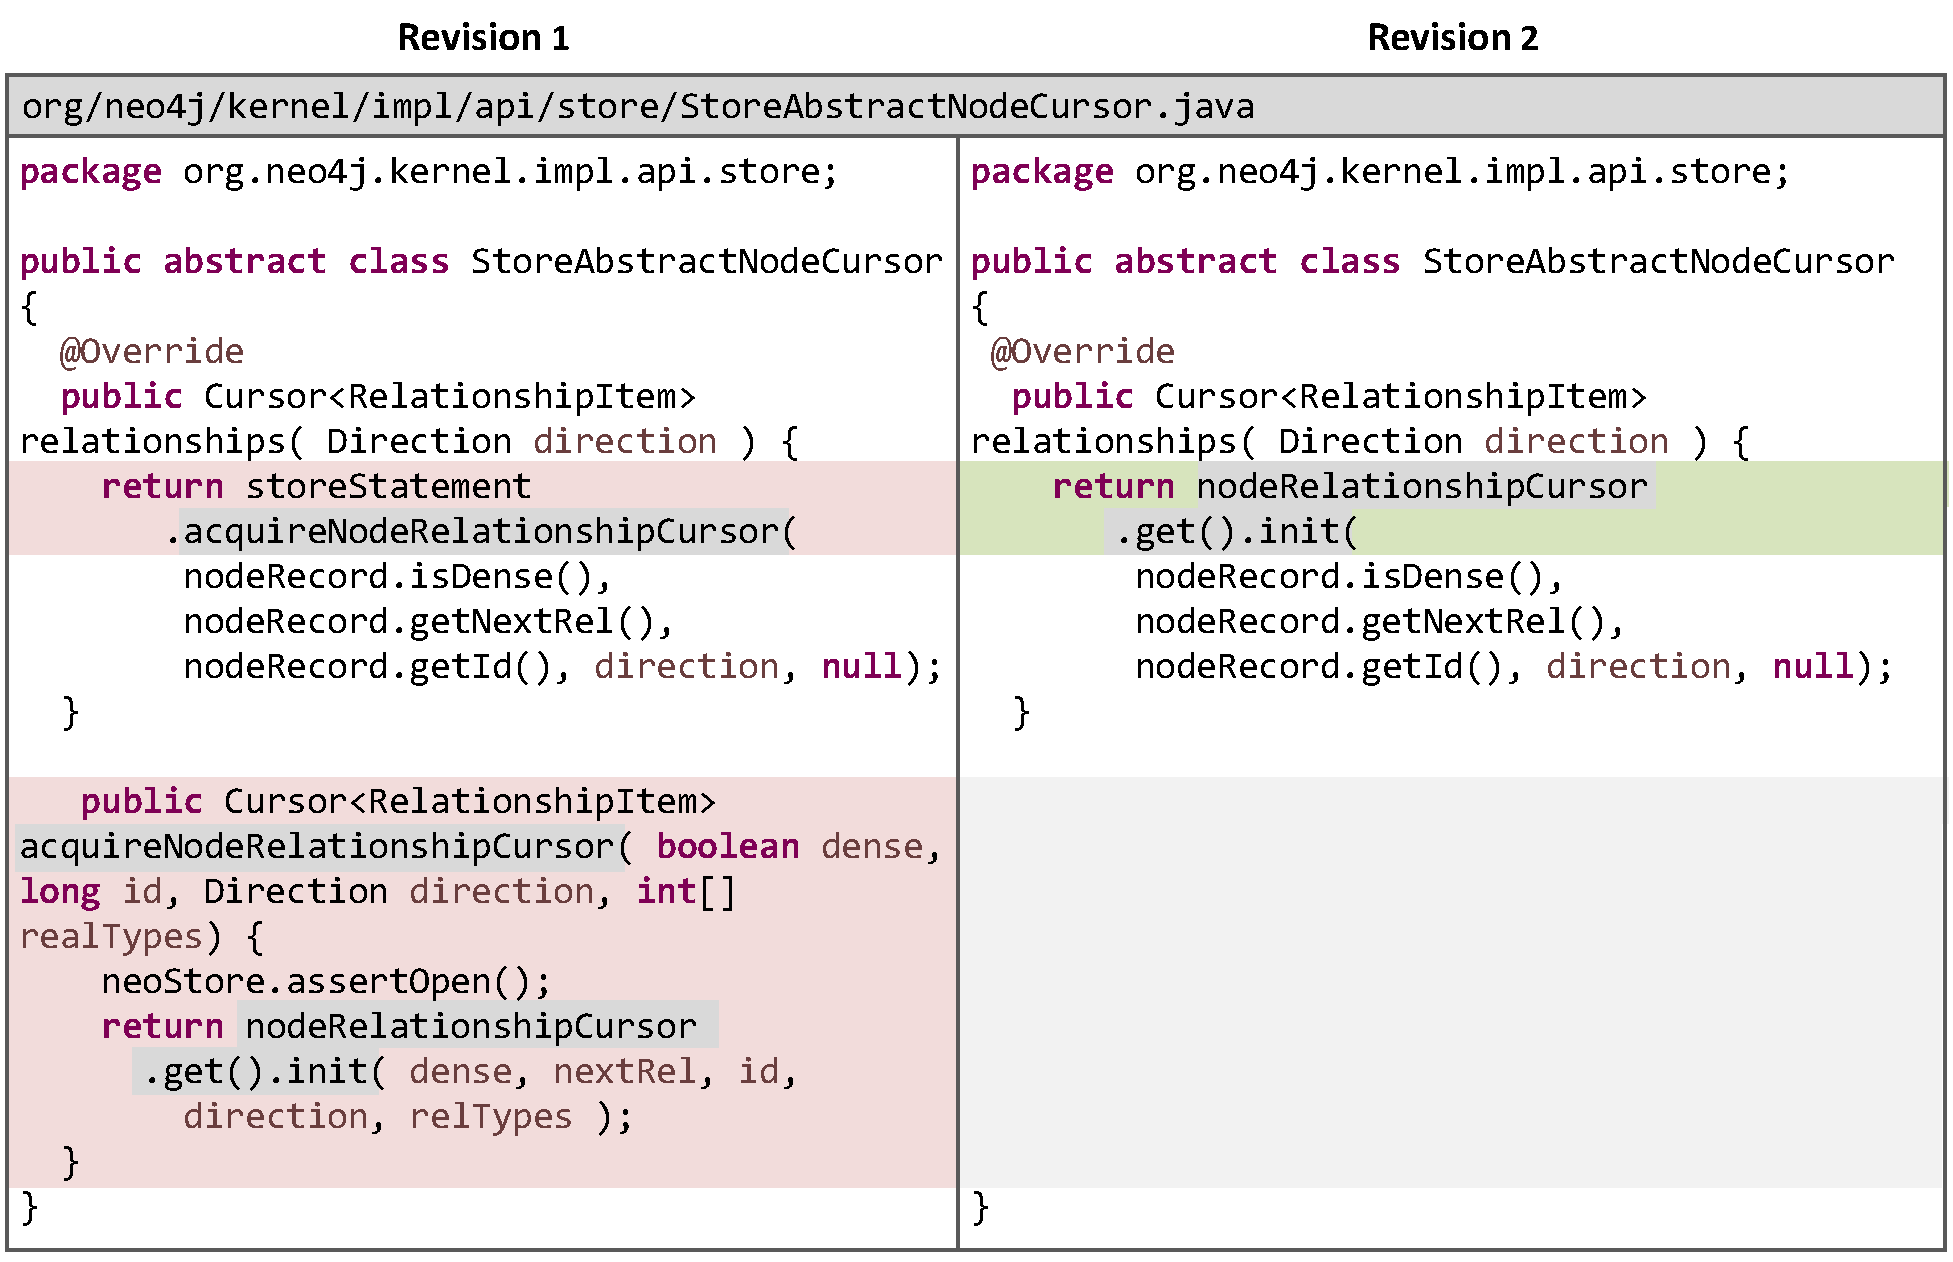
\includegraphics[width=0.8\textwidth]{img/diff2.pdf}
\caption{Illustrative diff of an \emph{Inline Method} refactoring considered as true positive by the validators.}
\label{FigDiff2}
\end{figure*}

After following this procedure, RefDiff 2.0 detected 278 new refactoring instances (i.e., not listed in the initial oracle), which were  validated by two paper's authors, called here validators. In the case of 173 refactorings (62\%), the validators agreed on their classification, including 115 refactorings labelled as true positives by both validators and 58 labelled as false positives. After this initial and independent validation, the validators discussed together the remaining 105 cases (38\%), to reach an agreement. As a result, 66 refactorings were considered true positives and 39 refactorings were classified as false positives. Figure~\ref{FigDiff2} shows a first example of true positive. RefDiff identified an \emph{Inline Method} refactoring, consisting on the substitution of the method named \codeinl{acquireNodeRelationshipCursor}, which was removed in the same commit, by invocations to methods \codeinl{get()} and \codeinl{init()}. We emphasize in this figure the changes that correspond to this refactoring. This indication of refactoring was not listed in the oracle. The validators individually analyzed this commit and both agreed that an \emph{Inline Method} was applied in this commit.



Figure~\ref{FigDiff3} shows another example of true positive, this time as an indication of \emph{Extract} and \emph{Move Method} refactorings. Developers removed the invocation to the method \codeinl{readValue(String, Class)}, which was extracted and moved to the class \codeinl{Controls}. An invocation to this new method \codeinl{validateControlsString(String)} was replaced in the same line. Similarly to the example in Figure~\ref{FigDiff2}, both validators agreed that \emph{Extract} and \emph{Move Method} were applied in this commit.

\begin{figure*}[htb]
\centering
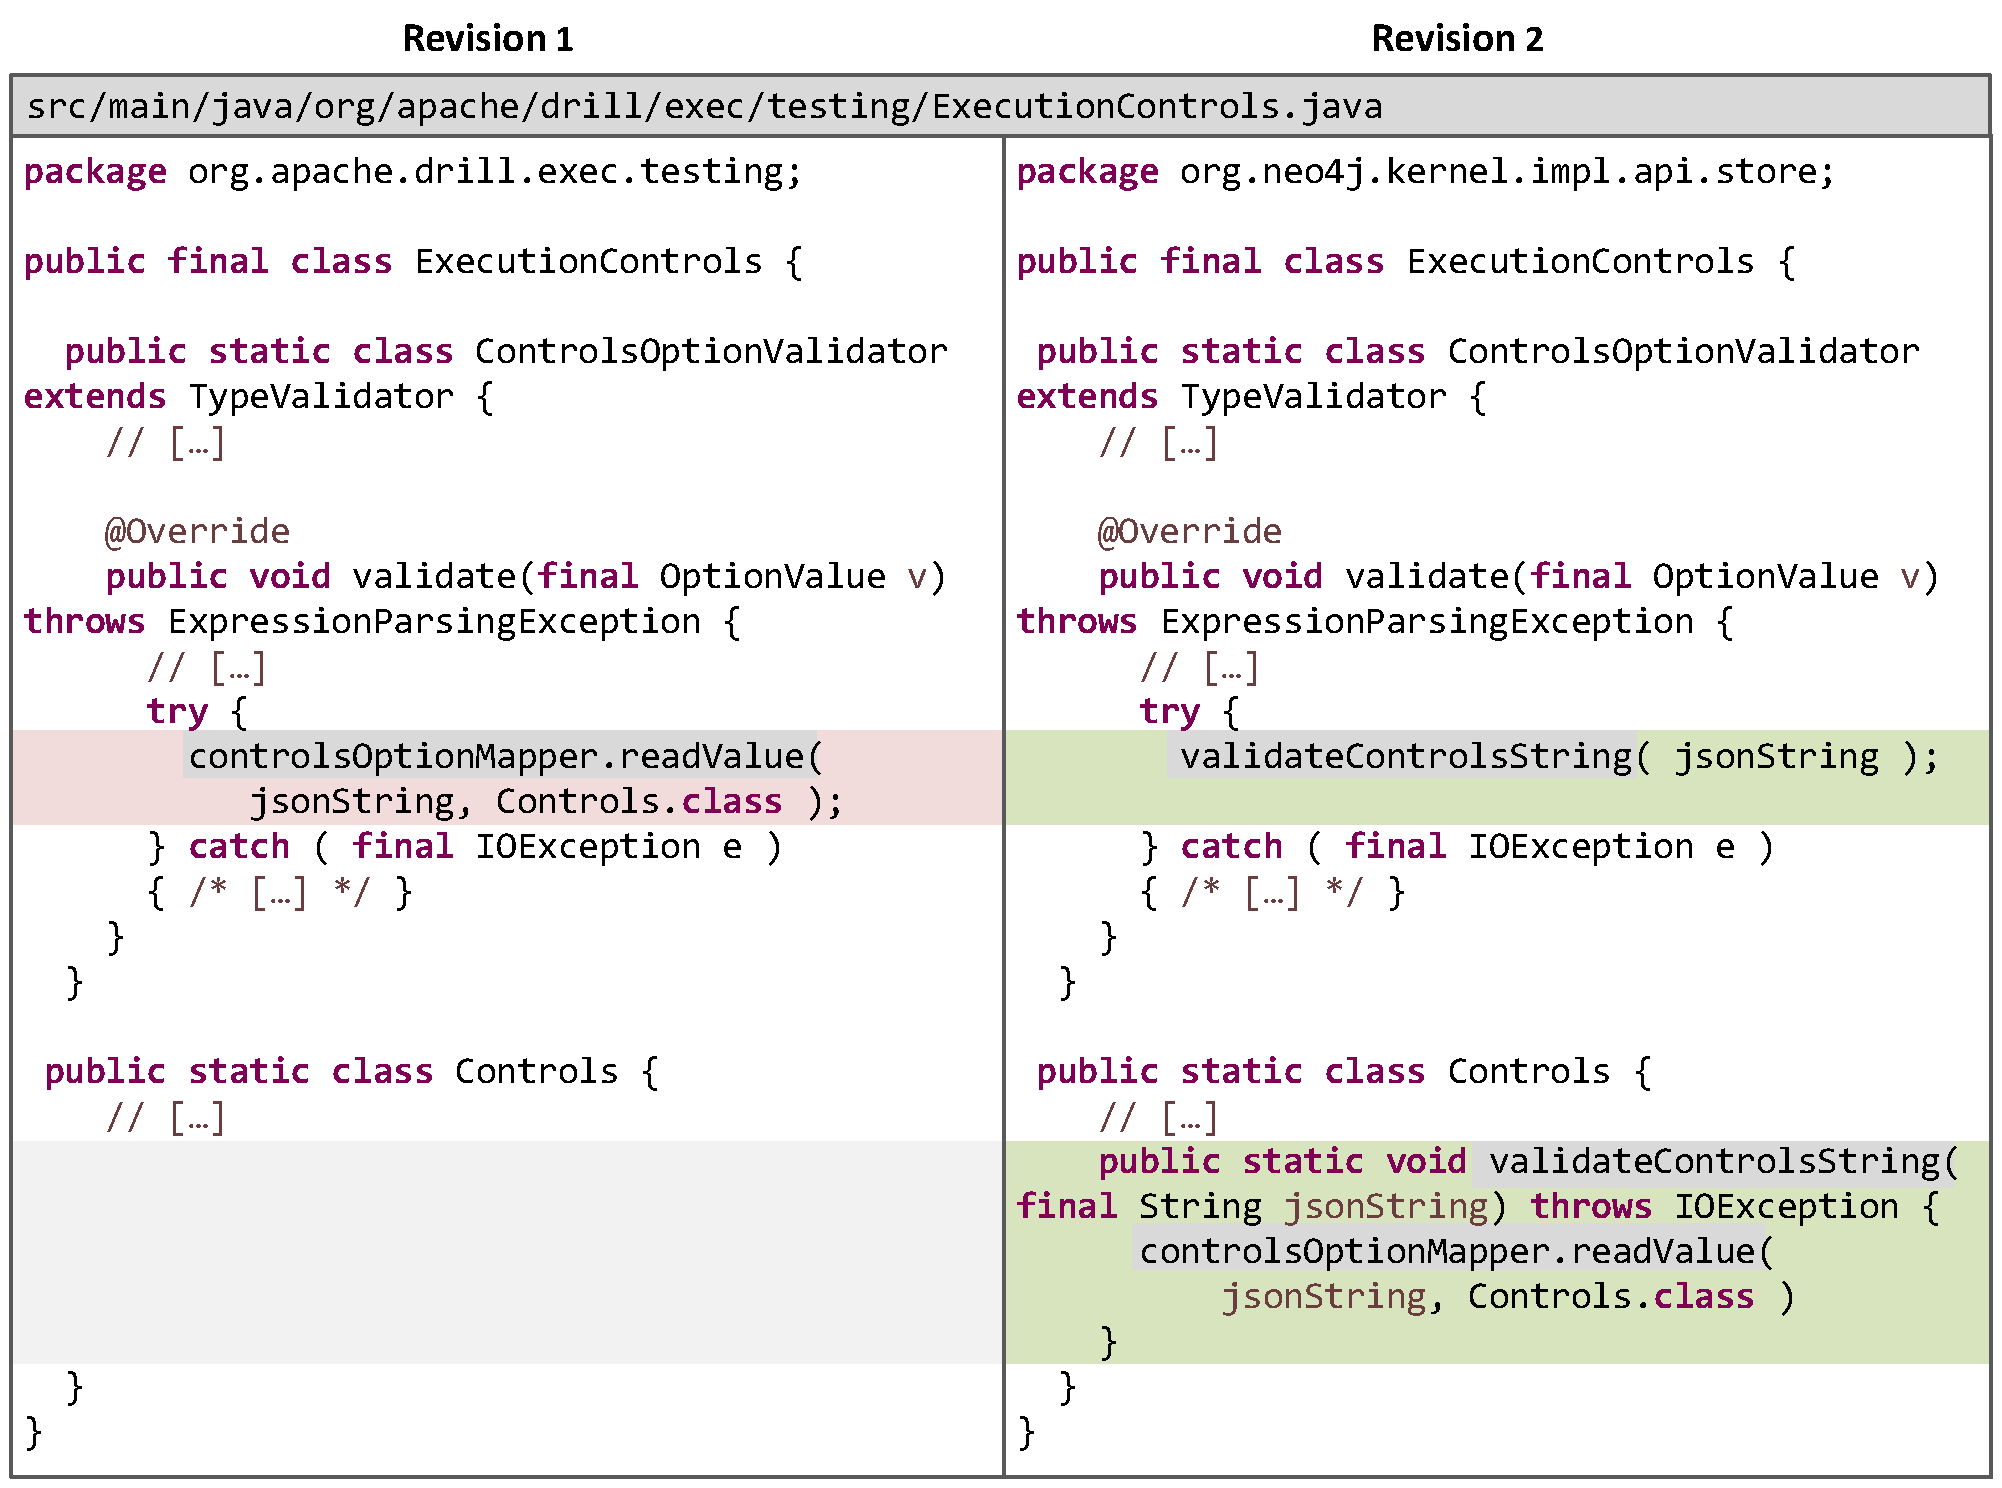
\includegraphics[width=0.8\textwidth]{img/diff3.pdf}
\caption{Illustrative diff of an \emph{Extract Method} refactoring considered as true positive by the validators.}
\label{FigDiff3}
\end{figure*}

After the manual validation of the refactoring instances it was possible to identify some common causes of failure.
In particular, one common reason for \emph{Move Method} false positives was missed \emph{Move/Rename Class}, i.e., RefDiff did not detect that the entire class has been moved (or renamed), and incorrectly reported that several of its members were moved.
We mitigated this issue by introducing a specific heuristic for this case (see Section~\ref{AlgoGeneral}).
Moreover, the analysis of the incorrect reports allowed us to identify and fix a couple of bugs in our implementation.
After applying the aforementioned fixes to RefDiff, it was necessary to run it again and compare the results against the update oracle. This time, 51 new refactoring instances were found, which were  validated by one of the authors. 24 of them (47\%) were classified as true positive, whilst 27 of them (53\%) were classified as false positive.

In summary, after these two rounds of manual validation, 184 new refactorings instances were classified as true positives and therefore included in the oracle.
The expanded oracle includes 3,261 refactoring instances (5.98\% more than the initial one) and it is publicly available at RefDiff's GitHub repository.\footnote{\url{https://github.com/aserg-ufmg/RefDiff}}

\subsection{Results}
\label{sec:eval:java:results}

\begin{table*}[htbp]
\renewcommand{\arraystretch}{1.2}
\caption{Java precision and recall results}
\label{TabResultJava}
\centering
\begin{tabular}{@{}lrlrrrlllrrrll@{}}
\toprule
 & & & \multicolumn{5}{c}{RefDiff} & & \multicolumn{5}{c}{Refactoring Miner}\\
\cmidrule{4-8} \cmidrule{10-14}
Refactoring Type & \# & & TP & FP & FN & Precision & Recall & & TP & FP & FN & Precision & Recall \\
\midrule
Move Class & 1121 & & 1067 & 1 & 54 & \xbar{0.999} & \xbar{0.952} & & 1017 & 0 & 104 & \xbar{1.000} & \xbar{0.907} \\
Move Method & 320 & & 256 & 38 & 64 & \xbar{0.871} & \xbar{0.800} & & 210 & 10 & 110 & \xbar{0.955} & \xbar{0.656} \\
Move and Rename/Rename Class & 92 & & 80 & 10 & 12 & \xbar{0.889} & \xbar{0.870} & & 59 & 1 & 33 & \xbar{0.983} & \xbar{0.641} \\
Rename Method & 346 & & 238 & 19 & 108 & \xbar{0.926} & \xbar{0.688} & & 270 & 6 & 76 & \xbar{0.978} & \xbar{0.780} \\
Extract Interface & 24 & & 21 & 3 & 3 & \xbar{0.875} & \xbar{0.875} & & 20 & 0 & 4 & \xbar{1.000} & \xbar{0.833} \\
Extract Superclass & 70 & & 52 & 0 & 18 & \xbar{1.000} & \xbar{0.743} & & 68 & 3 & 2 & \xbar{0.958} & \xbar{0.971} \\
Pull Up Method & 91 & & 75 & 2 & 16 & \xbar{0.974} & \xbar{0.824} & & 72 & 0 & 19 & \xbar{1.000} & \xbar{0.791} \\
Push Down Method & 40 & & 38 & 2 & 2 & \xbar{0.950} & \xbar{0.950} & & 33 & 0 & 7 & \xbar{1.000} & \xbar{0.825} \\
Extract/Extract and Move Method & 1037 & & 686 & 29 & 351 & \xbar{0.959} & \xbar{0.662} & & 796 & 12 & 241 & \xbar{0.985} & \xbar{0.768} \\
Inline Method & 120 & & 86 & 6 & 34 & \xbar{0.935} & \xbar{0.717} & & 97 & 1 & 23 & \xbar{0.990} & \xbar{0.808} \\
\addlinespace
Total & 3261 & & 2599 & 110 & 662 & \xbar{0.959} & \xbar{0.797} & & 2642 & 33 & 619 & \xbar{0.988} & \xbar{0.810} \\
\bottomrule
\end{tabular}
\end{table*}

Table~\ref{TabResultJava} shows the precision and recall results for RefDiff and RMiner using the oracle described in the previous section. The overall precision and recall of RefDiff is 95.9\% and 79.7\%, respectively.
Precision ranges from 87.1\% (\emph{Move Method}) to 100.0\% (\emph{Extract Superclass}), and it is above 90\% for 7 of the 10 refactoring types.
Recall ranges from 66.2\% (\emph{Extract Method}) to 95.2\% (\emph{Move Class}), and it is above 80\% for 6 of the 10 refactoring types.
On its turn, RMiner achieves 98.8\% of overall precision (ranging from 95.5\% to 100.0\%) and 81.0\% of overall recall (ranging from 64.1\% to 97.1\%).
When we analyze individual refactoring types, RefDiff's precision is always lower, but recall is higher in 6 refactoring types.
Thus, we conclude that both tools have very similar recall, but RMiner's precision is consistently higher.
Nevertheless, we argue that RefDiff's precision of 95.9\% is satisfactory, specially when we consider that our approach is programming language neutral.


\section{Evaluation with JavaScript and C}
\label{sec:eval:js:c:reults}

We also evaluate RefDiff with refactorings performed in two important but very different programming languages: JavaScript (a widely popular dynamic programming language, used mostly to build web applications) and C (a procedural programming language, used mostly to implement system software).
In the literature, we did not find a dataset with detailed information about real refactorings performed in these languages. Therefore, to evaluate precision, we manually validated the refactorings detected by RefDiff in a set of programs, in both languages (Section xx). Then, to evaluate recall, we created an oracle of manually validated refactoring operations performed in another set of programs (Section xx).  After that, in Section~\ref{sec:eval:js:c:results}, we report the precision and recall achieved by RefDiff.  We are not aware of any other tool for detecting refactorings in these languages. Therefore, in this second evaluation, it was not possible to compare RefDiff's results with competitor tools.

\subsection{Evaluation Design}
\label{sec:eval:js:c:design}

In this section, we defined the steps we followed to compute RefDiff's precision (Section~\ref{sec:eval:js:c:precision})
and recall (Section~\ref{sec:eval:js:c:recall}), when used to detect refactorings in JavaScript and C commits.

\subsubsection{Precision}
\label{sec:eval:js:c:precision}


To compute RefDiff's precision when detecting refactorings in JavaScript and C, we followed these steps:

\begin{enumerate}  
\item We selected the 20 most popular GitHub repositories of each language. For this, we queried the GitHub API for repositories, sorting by stars count---which is a reliable indicator of popularity in GitHub~\cite{icsme2016,jss-2018-github-stars} ---and filtering by programming language.
The resulting list of repositories was manually inspected to discard the ones that are not actual software projects, e.g., tutorials or code samples. Then, we forked each selected repository, to preserve their version histories from future changes pushed to the original project. Table xx shows the name, short description, and number of commits of each selected repository, both for JavaScrpit and C.  \todo{tabela que acabou de ser mencionada}

\item We ran RefDiff in the version history of each repository. To select the commits, we navigate the commit graph backwards, starting from the most recent commit in the master branch. We also discarded merge commits, i.e.,~commits which have two predecessors. The rationale is that comparing a merge commit with their predecessors results in duplicated reports of refactorings applied in the commits prior to the merge operation. Moreover, to avoid over-representing projects with longer histories, we established a limit of 500 commits per repository. For each selected commit, we compared its source code with its predecessor using RefDiff, to detect refactoring operations.

\item Given the list of refactorings detected by RefDiff, we randomly selected 10 instances of each refactoring type to manually assess whether they correspond to actual refactorings (true positives), or incorrect reports (false positives).
When applying the random selection, we enforced the constraint that we should not select two refactoring instances performed in the same commit.
In this way, we avoid selecting similar refactorings which were performed in batch, e.g., multiple classes or functions moved together.
To confirm each refactoring instance, one of the authors manually inspected the diff of the code changes in the corresponding commit.
\end{enumerate}

After following the three steps, we compute precision as $P = \mathit{TP} / (\mathit{TP} + \mathit{FP})$, where $\mathit{TP}$ is the number of true positives and $\mathit{FP}$ is the number of false positives.



\subsubsection{Recall}
\label{sec:eval:js:c:recall}

To compute RefDiff's recall when detecting refactorings in JavaScript and C, we followed three steps:

\begin{enumerate}  
\item We used GitHub API to find refactorings documented in commits from the repositories selected for evaluating precision (Section~\ref{sec:eval:js:c:precision}). Such queries consist in searching for keywords denoting a particular type of refactoring in the commit message, as described in Table xx.\todo{acrescentar esta tabela} For example, when looking for \emph{Rename Function} refactoring instances in JavaScript, we built a query that looks for commits which contain the keywords \texttt{rename} and \texttt{function} in their messages.

\item Given the results of a query, we manually inspected the commit message and the diff of the source code to confirm the applied refactoring. We repeated this procedure until we found 10 instances of each refactoring type or when there were no more results to inspect (which happened only for xxx \todo{detalhar refactorings com menos de 10 instances)}. Each confirmed refactoring was recorded in a normalized textual format compatible with the output of RefDiff.

%It is worth noting that, during this procedure, most of the results were discarded because the commit message did not actually documented a refactoring. Besides, the diff of some of the commits were so large that could not be displayed in the user interface. In summary, we only registered the refactoring instances that we could confirm both in the commit message and in the code diff.

\item We ran RefDiff in the commits that contain documented and manually-validated refactorings to assess whether they are reported (true positives) or missed (false negatives). 

\end{enumerate}

After following these steps, we compute recall as $R = \mathit{TP} / (\mathit{TP} + \mathit{FN})$, where $\mathit{TP}$ is the number of true positives and $\mathit{FN}$ is the number of false negatives.


\subsection{Results}
\label{sec:eval:js:c:results}

In this section, we present the precision and recall results for JavaScript (Section~\ref{sec:eval:js:c:results:js}) and C (Section xx).

\subsubsection{JavaScript Results}
\label{sec:eval:js:c:results:js}

Table~\ref{TabResultJsPrecison} shows the precision results for JavaScript. The overall precision is 91\%. There are three refactorings with precision of 80\%: Rename Function, Move and Rename Function, and Inline Function. For the remaining refactoring types, RefDiff has as precision of 90\% (two refactoring types) or a precision of 100\% (five refactoring types). Table~\ref{TabResultJsRecall} shows the recall results, which reach 88\% when all refactoring types are considered together.
Inline function has the lowest recall (40\%); however, in our oracle has only five instances of this operation. The two most common refactorings (Move File and Move Function, both with 10 instances) have a recall of 100\%.

%The following GitHub repositories were selected to run evaluation procedure:
%\textsc{facebook/\-react}, 
%\textsc{vuejs/\-vue}, 
%\textsc{d3/\-d3}, 
%\textsc{face\-book/\-react-native}, 
%\textsc{angular/\-angular.js}, 
%\textsc{face\-book/\-create-react-app}, 
%\textsc{jquery/\-jquery}, 
%\textsc{atom/\-atom}, 
%\textsc{axios/\-axios}, 
%\textsc{mrdoob/\-three.js}, 
%\textsc{socketio/\-socket.io}, 
%\textsc{reduxjs/\-redux}, 
%\textsc{webpack/\-webpack}, 
%\textsc{Semantic-Org/\-Semantic-UI}, 
%\textsc{hakimel/\-reveal.js}, 
%\textsc{meteor/\-meteor}, 
%\textsc{expressjs/\-express}, 
%\textsc{mui-org/\-material-ui}, 
%\textsc{chartjs/\-Chart.js}


\begin{table}[htbp]
\renewcommand{\arraystretch}{1.2}
\caption{JavaScript precision results}
\label{TabResultJsPrecison}
\centering
\begin{tabular}{@{}lrrl@{}}
\toprule
Refactoring Type & TP & FP & Precision\\
\midrule
Move File & 10 & 0 & \xbar{1.00} \\
Move Class & 2 & 0 & \xbar{1.00} \\
Move Function & 9 & 1 & \xbar{0.90} \\
Rename File & 10 & 0 & \xbar{1.00} \\
Rename Class & 5 & 0 & \xbar{1.00} \\
Rename Function & 8 & 2 & \xbar{0.80} \\
Move and Rename File & 10 & 0 & \xbar{1.00} \\
Move and Rename Function & 8 & 2 & \xbar{0.80} \\
Extract Function & 9 & 1 & \xbar{0.90} \\
Inline Function & 8 & 2 & \xbar{0.80} \\
\addlinespace
Total & 79 & 8 & \xbar{0.91} \\
\bottomrule
\end{tabular}
\end{table}

\begin{table}[htbp]
\renewcommand{\arraystretch}{1.2}
\caption{JavaScript recall results}
\label{TabResultJsRecall}
\centering
\begin{tabular}{@{}lrrl@{}}
\toprule
Refactoring Type & TP & FN & Recall\\
\midrule
Move File & 10 & 0 & \xbar{1.00} \\
Move Function & 10 & 0 & \xbar{1.00} \\
Rename File & 8 & 2 & \xbar{0.80} \\
Rename Function & 9 & 1 & \xbar{0.90} \\
Move and Rename File & 3 & 0 & \xbar{1.00} \\
Move and Rename Function & 6 & 1 & \xbar{0.86} \\
Extract Function & 9 & 1 & \xbar{0.90} \\
Inline Function & 2 & 3 & \xbar{0.40} \\
\addlinespace
Total & 57 & 8 & \xbar{0.88} \\
\bottomrule
\end{tabular}
\end{table}


\subsection{C evaluation results}

The following GitHub repositories were selected to run evaluation procedure:
\textsc{torvalds/\-linux}, 
\textsc{firehol/\-netdata}, 
\textsc{antirez/\-redis}, 
\textsc{git/\-git}, 
\textsc{Bilibili/\-ijkplayer}, 
\textsc{php/\-php-src}, 
\textsc{wg/\-wrk}, 
\textsc{ggreer/\-the\_silver\_searcher}, 
\textsc{kripken/\-emscripten}, 
\textsc{vim/\-vim}, 
\textsc{stedolan/\-jq}, 
\textsc{FFmpeg/\-FFmpeg}, 
\textsc{tmux/\-tmux}, 
\textsc{vurtun/\-nuklear}, 
\textsc{obsproject/\-obs-studio}, 
\textsc{libuv/\-libuv}, 
\textsc{swoole/\-swoole-src}, 
\textsc{curl/\-curl}, 
\textsc{irungentoo/\-toxcore}, 
\textsc{pjreddie/\-darknet} 


\begin{table}[htbp]
\renewcommand{\arraystretch}{1.2}
\caption{C precision results}
\label{TabResultCPrecison}
\centering
\begin{tabular}{@{}lrrl@{}}
\toprule
Refactoring Type & TP & FP & Precision\\
\midrule
Move File & 10 & 0 & \xbar{1.00} \\
Move Function & 8 & 2 & \xbar{0.80} \\
Rename File & 10 & 0 & \xbar{1.00} \\
Rename Function & 9 & 1 & \xbar{0.90} \\
Move and Rename Function & 8 & 2 & \xbar{0.80} \\
Change Signature & 10 & 0 & \xbar{1.00} \\
Extract Function & 10 & 0 & \xbar{1.00} \\
Inline Function & 5 & 5 & \xbar{0.50} \\
\addlinespace
Total & 70 & 10 & \xbar{0.88} \\
\bottomrule
\end{tabular}
\end{table}


\begin{table}[htbp]
\renewcommand{\arraystretch}{1.2}
\caption{C recall results}
\label{TabResultCRecall}
\centering
\begin{tabular}{@{}lrrl@{}}
\toprule
Refactoring Type & TP & FN & Recall\\
\midrule
Change Signature & 9 & 1 & \xbar{0.90} \\
Extract Function & 7 & 3 & \xbar{0.70} \\
Inline Function & 9 & 1 & \xbar{0.90} \\
Move File & 10 & 0 & \xbar{1.00} \\
Move Function & 8 & 2 & \xbar{0.80} \\
Move and Rename File & 10 & 0 & \xbar{1.00} \\
Move and Rename Function & 9 & 1 & \xbar{0.90} \\
Rename File & 10 & 0 & \xbar{1.00} \\
Rename Function & 10 & 0 & \xbar{1.00} \\
\addlinespace
Total & 82 & 8 & \xbar{0.91} \\
\bottomrule
\end{tabular}
\end{table}


